\chapter{Results}\label{sec:results}

In this chapter, the proposed experimens are presented and explained. For each experiment, the results are showed and discussed.
There is total of five proposed experiments:
\begin{itemize}[itemsep=0.1cm]
    \item \textbf{Experiment 1 - Preliminary Experiment:} aims to demonstrate the necessity of Hyperparameter Optimization (HPO) and to familiarize with the concepts of HPO.
    \item \textbf{Experiment 2 - Comparison of Optuna's Samplers on MNIST:} aims to evaluate the performance of different Hyperparameter Optimization algorithms, specifically Optuna's Samplers, on the MNIST dataset.
    \item \textbf{Experiment 3 - Comparison between a Custom PSO implementation and Optuna:} aims to compare the performance of a custom implementation of Particle Swarm Optimization (PSO) with Optuna's Samplers, on the MNIST dataset.
    \item \textbf{Experiment 4 - Comparison between a PSO Sampler and Optuna's Samplers:} aims to compare the performance of a PSO Sampler (made using Optuna as a base) with the other Optuna's Samplers, on the MNIST dataset.
    \item \textbf{Experiment 5 - Hyperparameter Optimization on Weed Map Dataset:} aims to perform Hyperparameter Optimization on the Weed Map Dataset, using Optuna.
\end{itemize}

\myparagraph{Experiments Source Code:}
All the source code of the experiments is available on the same repository \cite{Repository-THESIS} mentioned in the previous chapther (Chapter~\ref{sec:methodology}), specifically in the \texttt{/experiments/} package.
In particular, the Weed Map Experiment (Experiment 5) is in the file \newline\texttt{/weed\_mapping\_experiment/Weed\_Mapping\_Optimization.ipynb}, while the other experiments were run using \texttt{/MNIST\_experiment/MNIST\_Optimization.ipynb}.

\section{Experiment 1 - Preliminary Experiment}

This Preliminary Experiment has a double goal.
The first is to familiarize with the concepts of HPO also from a physical implementation perspective.
The second reason is to establish, if ever needed, the necessity of Hyperparameter Optimization; to demonstrate that HPO can actually improve the final performance of a ML experiment by finding the best Hyperparameters to train the model object of the experiment.
\\[0.3cm]Note that in this preliminary experiment, everything was developed with simple vanilla Python, without the use of the infrastructure described in the previous chapter (Chapter~\ref{sec:methodology}).

\myparagraph{Hardware used for the Experiment:}
The hardware which was utilized to run this experiment is the following:
\begin{itemize}[itemsep=0.1cm]
    \item CPU: Intel Core i5-8265U CPU @ 1.60GHz (4-core, 8 thread)
    \item GPU: NVIDIA GeForce MX 110 (2GB VRAM)
    \item RAM: 8GB (DDR4)
    \item Disk: SSD
    \item OS: Windows 11
\end{itemize}

\subsection{Preparation of the Experiment}

Given the first goal of the experiment, the idea is to realize a simple implementation of the most traditional of HPO Algorithms, which is Grid Search.
\\[0.3cm]The first part of the experiment consist in recreating another ML experiment which does not apply HPO and evaluate its results. Successively, the hyperparameters of that same ML model will be optimized with the custom Grid Search.
\\[0.3cm]The experiment chosen for comparison is the one proposed by the book “Dive Into Deep Learning” \cite{Tesi-1.6} (chapter 4 of the book). Some modifications have been made to this experiment: firstly, a simpler version of the proposed dataset is used, then the Multi-Layer Perceptron (MLP) considered is implemented with vanilla Python rather than PyTorch.

\myparagraph{Dataset of the Experiment:}
The Dataset considered for the experiment is a simplified version of MNIST, specifically, the version included in scikit-learn \cite{scikit-learn}, from the function \texttt{load\_digits()} of the dataset module. (An explanation of the complete MNIST dataset is in the following experiment; for this preliminary experiment is not necessary to understand the dataset).

\myparagraph{Choice of Model and Hyperparameters:}
As introduced earlier, the MLP model utilized is not the same as the one from the book. This is not detrimental to the scientific value of the experiment, as the considered hyperparameters and configuration of the model were the same proposed in the book, so that a comparison would still be possible.

\myparagraph{Implementation of Grid Search:}
The proposed implementation of Grid Search is completely made from scratch.
The algorithm takes as input the model, the dataset and the grid of hyperparameters; the grid is a Python \texttt{dict}, where \texttt{keys} are \texttt{str} which represent the name of the hyperparameter, and \texttt{values} are \texttt{list} which contain the values that the corresponding hyperparameter can be.
\\[0.3cm]At the start of the algorithm, a Cartesian Product in applied on the lists inside the \texttt{param\_grid}, basically generating all the trials that are going to be evaluated.
For each trial, the model is initialized with the hyperparameters of that trial and is evaluated; the results are saved in a variable.
After having completed all the trials, the algorithm returns as output the variable containing all the results, from which it can be obtained the best trial.
\\[0.3cm]Two versions of this algorithm have been developed, one without and one with parallelism. There is no difference between the two, the only one is that the second allows to execute multiple trials on multiple threads.

\subsection{Execution of the Experiment}

The execution of the experiment divides in three short parts: run and evaluation without hyperparameter optimization; run and evaluation with hyperparameter optimization; comparison of results.
\\[0.3cm]The set of hyperparameter utilized by the book for the experiment are the following:
\begin{itemize}[itemsep=0.1cm]
    \item Activation Input: Sigmoid
    \item Activation Output: Softmax
    \item Batch Size: 256
    \item Learning Rate: 0.1
    \item Hidden Size: 10
    \item Epochs: 10000
\end{itemize}
Training and evaluating the model with these hyperparameter lead to the results of 99\% of accuracy on the Training Set and 97\% on the Test Set.
The custom Grid Search algorithm is executed with the \texttt{param\_grid} in the figure (Fig.~\ref{fig:figure-4.1.1}) as input.
\begin{figure}[t]
	\centering
	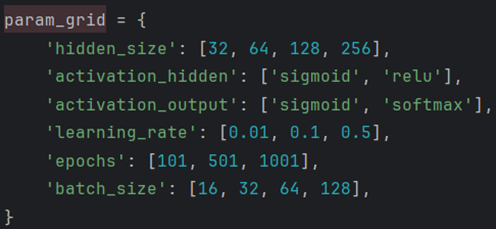
\includegraphics[width=8cm]{figures/figure-4.1.1.png}
	\caption[Param Grid for Custom Grid Search Experiment]{The Param Grid utilized for the Custom Grid Search Experiment.}
	\label{fig:figure-4.1.1}
\end{figure}
\\[0.3cm]The Grid Search algorithm executed a total of 576 trials. After the completion of the Optimization, there are three best results (with the same accuracy), which are in the figure (Fig.~\ref{fig:figure-4.1.2}).
\begin{figure}[t]
	\centering
	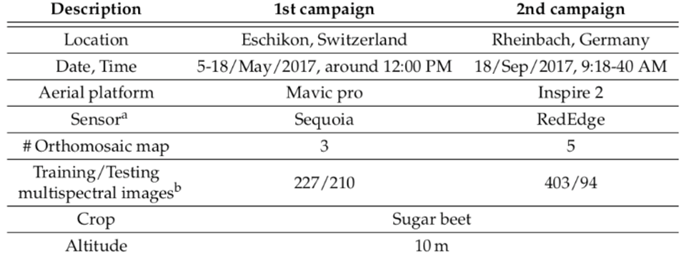
\includegraphics[width=15cm]{figures/figure-4.1.2.png}
	\caption[Best Results of Custom Grid Search Experiment]{The three best results of the Custom Grid Search Experiment.}
	\label{fig:figure-4.1.2}
\end{figure}
\\[0.3cm]These best results have an accuracy of 100\% on the Training Set and 98.6\% on the Test Set. Moreover, there are more than 20 trials with a better accuracy than the configuration proposed by the book.

\subsection{Discussion of the Results}

This simple experiment with its results outlines how hyperparameter optimization, even when using an simple implementation of the weakest algorithm, could lead to a signification improvement in the performance of the trained model.
\\[0.3cm]The gained 1.6\% accuracy on the Test Set may seem a little improvement, but is remarkable, especially when the dataset is composed by a very large number of observations.
\\[0.3cm]These results, additionally, also confirm another aspect of HPO, that is the ability of improving the performance of an experiment without interfering with the model or the dataset.

\section{Experiment 2 - Comparison of Optuna's Samplers on MNIST}

The objective of this experiment is to evaluate the performance of different Hyperparameter Optimization algorithms so as to gain general knowledge about the capacity of each in preparation for subsequent more complex experiments.
\\[0.3cm]In order to make the results and the methodology the most scientifically comparable as possible, rather than implementing various Samplers from scratch singularly, a library for HPO is used.
\\[0.3cm]The chosen library is Optuna, which as described in previous sections, includes a few Samplers already implemented, with the same style and same preconditions, making each optimization perfectly comparable to one other.
\\[0.3cm]As the idea is to have results which are the most general as possible, and because such “optimization of optimizations” is inevitably enormously expensive, a simple dataset is considered, which is MNIST.

\myparagraph{Hardware used for the Experiment:}
The hardware which was utilized to run this experiment is the following:
\begin{itemize}[itemsep=0.1cm]
	\item CPU: Intel Core i7-10700K CPU @ 3.80GHz
	\item GPU: NVIDIA GeForce RTX 3080 (10GB VRAM)
	\item RAM: 16GB (DDR5)
	\item Disk: SSD
	\item OS: Linux (Ubuntu)
\end{itemize}

\subsection{MNIST Dataset}

The MNIST Dataset is a database of images of handwritten digits \cite{MNIST}.
MNIST is the ideal dataset for learners and for small experiments regarding the field pattern recognition, is basically a benchmarking dataset for Image Classification.
\\[0.3cm]Each image of the MNIST Dataset represent a digit from 0 to 9, making it ideal for benchmarking simple classification models for images (Fig.~\ref{fig:figure-4.1.3}).
\begin{figure}[t]
	\centering
	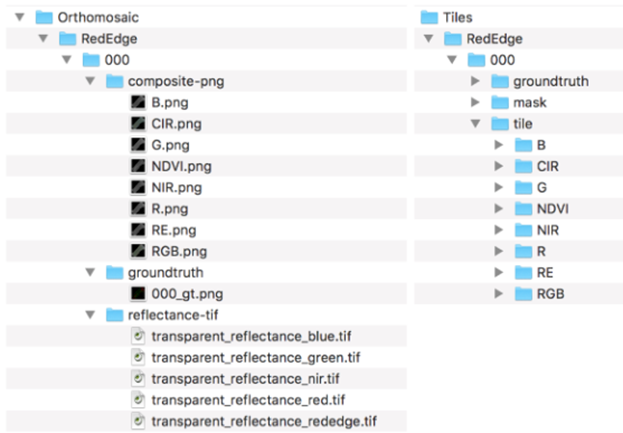
\includegraphics[width=9cm]{figures/figure-4.1.3.png}
	\caption[Examples of MNIST Images]{Some examples of images in the original MNIST dataset. Source:~\cite{MNIST}}
	\label{fig:figure-4.1.3}
\end{figure}

\subsubsection{Structure of MNIST Dataset}

The MNIST Dataset is composed of a total of 70000 images, of which 60000 are part of the training set and 10000 are part of the test set \cite{MNIST}.
The total wight of MNIST is 11.6MB when compressed, 52.3MB normally. Each image is 28x28 pixels, is in black and white, and weights 784 bytes.

\myparagraph{NIST Dataset:}
MNIST is a newer version of an old dataset called NIST, in which the division was between SD-1 (Special Database 1) and SD-3 (Special Database 3). Where SD-3 was the training set, and SD-1 the test set. The images of SD-3 were much clearer and easier to recognize.
\\[0.3cm]MNIST is designed so that half of its training images and half of its test images come from SD-1 and the remaining half from SD-3.
This means that half of the images of MNIST are easier to recognize, the other half are more difficult.

\subsubsection{Variants of MNIST Dataset}
Given its extreme simplicity to both use and understand, MNIST has inspired numerous variants. Some of the most famous variants are the following:
\begin{itemize}[itemsep=0.1cm]
    \item \textbf{Fashion-MNIST:} replaces digits with images of clothing items to test models on more complex visual patterns (Fig.~\ref{fig:figure-4.1.4}).
    \begin{figure}[t]
		\centering
		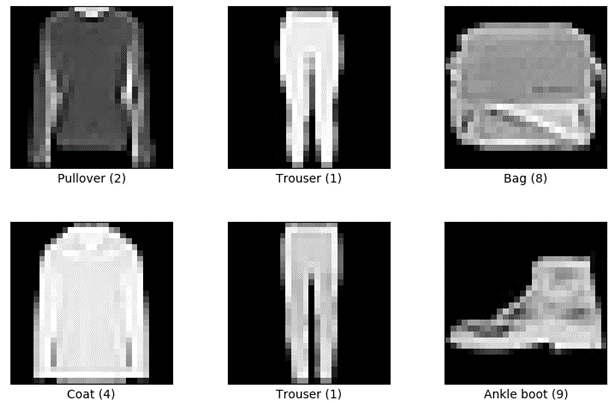
\includegraphics[width=10cm]{figures/figure-4.1.4.png}
		\caption[Examples of Fashion-MNIST Images]{Some examples of images in the Fashion-MNIST dataset. Source: Google Images}
		\label{fig:figure-4.1.4}
	\end{figure}
	\item \textbf{EMNIST (Extended MNIST):} includes, in addition to digits, also letters, to enhance the diversity of the dataset.
    \item \textbf{KMNIST:} includes images of Japanese Kanji characters, making the classification task much more complex than the version on the Latin alphabet.
    \item \textbf{NoiseMNIST:} is a version on MNIST where Gaussian noise is added to the images, it is useful to test the robustness of the model against noisy data.
    \item \textbf{Rotated MNIST:} is a version of MNIST where the images are rotated by a random angle, to test the robustness of the model against rotated data.
\end{itemize}
% 
% \myparagraph{Fashion-MNIST:}
% Fashion-MNIST replaces digits with images of clothing items to test models on more complex visual patterns.
% \begin{figure}[t]
% 	\centering
% 	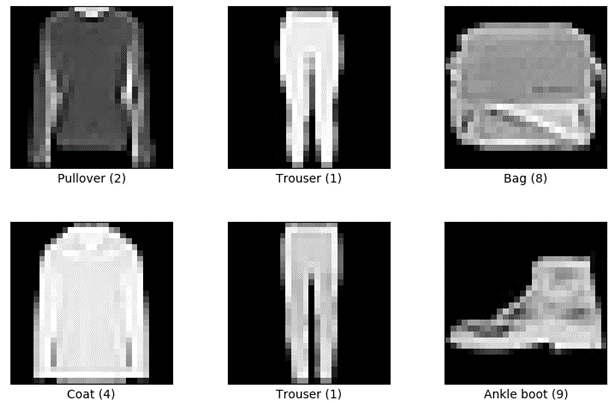
\includegraphics[width=15cm]{figures/figure-4.1.4.png}
% 	\caption[Examples of Fashion-MNIST Images]{Some examples of images in the Fashion-MNIST dataset. Source: Google Images}
% 	\label{fig:figure-4.1.4}
% \end{figure}
% 
% \myparagraph{EMNIST (Extended MNIST):}
% EMNIST includes, in addition to digits, also letters, to enhance the diversity of the dataset.
% 
% \myparagraph{KMNIST:}
% KMNIST includes images of Japanese Kanji characters, making the classification task much more complex than the version on the Latin alphabet.
% 
% \myparagraph{NoiseMNIST:}
% NoiseMNIST is a version on MNIST where Gaussian noise is added to the images, it is useful to test the robustness of the model against noisy data.

\subsection{Preparation of the Experiment}

\subsection{Execution of the Experiment}

\subsection{Discussion of the Results}

\section{Experiment 3 - Comparison between a Custom PSO implementation and Optuna}

\myparagraph{Hardware used for the Experiment:}
The hardware which was utilized to run this experiment is the same as Experiment 2.

\subsection{Preparation of the Experiment}

\subsection{Execution of the Experiment}

\subsection{Discussion of the Results}

\section{Experiment 4 - Comparison between a PSO Sampler and Optuna's Samplers}

\myparagraph{Hardware used for the Experiment:}
The hardware which was utilized to run this experiment is the same as Experiment 2.

\subsection{Preparation of the Experiment}

\subsection{Execution of the Experiment}

\subsection{Discussion of the Results}

\section{Experiment 5 - Hyperparameter Optimization on Weed Map Dataset}

\myparagraph{Hardware used for the Experiment:}
The hardware which was utilized to run this experiment is the following:
\begin{itemize}[itemsep=0.1cm]
	\item CPU: AMD EPYC 7V12(Rome) @ 2.45GHz (4-core)
	\item GPU: NVIDIA Tesla T4 (16GB VRAM)
	\item RAM: 28GB
	\item Disk: SSD
	\item OS: Linux (Ubuntu)
\end{itemize}
(This hardware is a Virtual Machine on the Azure ML servers).

\subsection{Weed Map Dataset}

\subsubsection{Introduction to Weed Map Dataset}

Weed Map Dataset is the dataset for the research “WeedMap: A large-scale semantic weed mapping framework using aerial multispectral imaging and deep neural network for precision farming” \cite{Tesi-2.1}.
\\[0.3cm]Each picture of the Dataset shows an image of a cultivated field, where there can been distinguished Dirt, Weeds and Crops.
\\[0.3cm]The image below (Fig.~\ref{fig:figure-4.5.1}) is an example on one of the images. It is first showed the entire Orthomosaic Map, and then different zoom levels. This puts in evidence the large scale of the image and the difficulty in distinguishing between Crops and Weeds.
\begin{figure}[t]
	\centering
	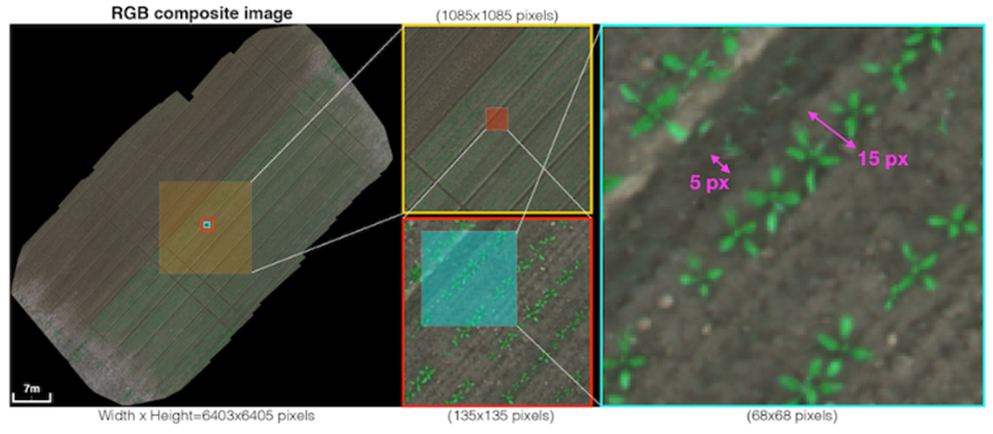
\includegraphics[width=14cm]{figures/figure-4.5.1.png}
	\caption[Example of image in Weed Map Dataset]{Example of image in Weed Map Dataset; with different zoom levels. Source:~\cite{Tesi-2.1}}
	\label{fig:figure-4.5.1}
\end{figure}

\myparagraph{Data Collection:}
The data included in the dataset was collected from aerial images (with Drones) from two different Sugar Beet fields: Eschikon (Switzerland) and Rheinbach (Germany). (Fig.~\ref{fig:figure-4.5.2})
\\[0.3cm]In particular, the utilized Drones are two commercial quadrotor UAV, equipped with multispectral cameras.
\begin{figure}[t]
	\centering
	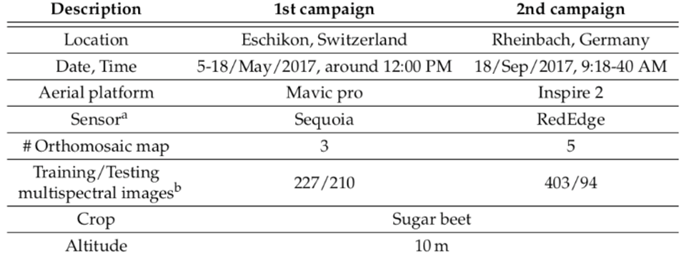
\includegraphics[width=13cm]{figures/figure-4.5.2.png}
	\caption[Information on Campaigns of Weed Map Dataset]{Information on the campaigns of data collection of Weed Map Dataset. Source:~\cite{Tesi-2.1}}
	\label{fig:figure-4.5.2}
\end{figure}

\subsubsection{Structure of Weed Map Dataset}

The full Dataset consist of 129 Directories for a total of 18746 images files. The total weight is 5.36GB.

\myparagraph{Folder Structure:}
There are two main folders, which are Orthomosaic and Tiles.
Orthomosaic contains the full orthomosaic maps.
Tiles contains, for each orthomosaic map, a folder containing images which represents cropped sections of the original orthomosaic map. All cropped sections together form the full map.
\\[0.3cm]Both Orthomosaic and Tiles contain RedEdge and Sequoia subfolders, containing 8 Orthomosaic maps in total (5 RedEdge and 3 Sequoia). (Fig.~\ref{fig:figure-4.5.3})
\\[0.3cm]Each Orthomosaic map stand in a folder indexed 000 to 007.
\begin{figure}[t]
	\centering
	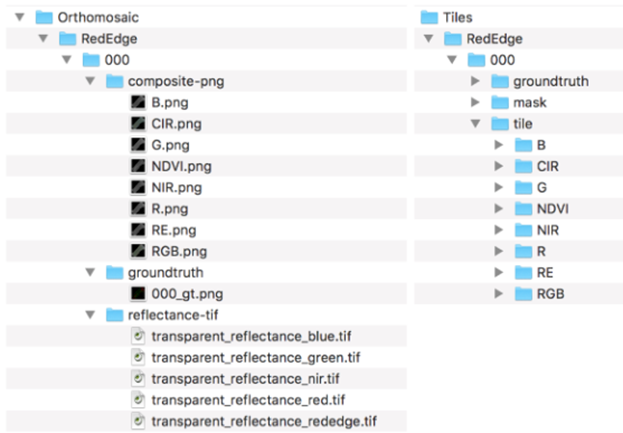
\includegraphics[width=10cm]{figures/figure-4.5.3.png}
	\caption[Folder Structure Weed Map Dataset]{Table showing the folder structure of Weed Map Dataset. Source:~\cite{Tesi-2.1}}
	\label{fig:figure-4.5.3}
\end{figure}

\myparagraph{Groundtruth:}
The Groundtruth images are pictures of the fields where each pixel has been manually labelled. (Fig.~\ref{fig:figure-4.5.4})
Each class is represented in a different colour:
\begin{itemize}[itemsep=0.1cm]
	\item Background (Dirt and part and part of the image which is not the crop field): is Black (code 0)
	\item Crops: is Green (code 1)
	\item Weeds: is Red (code 2)
\end{itemize}
The Groundtruth images are utilized to evaluate the precision of each prediction.
\begin{figure}[t]
	\centering
	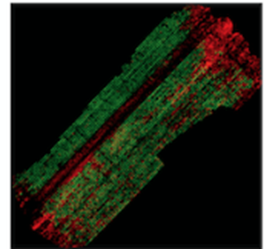
\includegraphics[width=5cm]{figures/figure-4.5.4.png}
	\caption[Example of GroundTruth in Weed Map Dataset]{Example of GroundTruth image in Weed Map Dataset. Source:~\cite{Tesi-2.1}}
	\label{fig:figure-4.5.4}
\end{figure}

\subsection{Preparation of the Experiment}

\subsection{Execution of the Experiment}

\subsection{Discussion of the Results}


